\chapter{Theoretical Fundamentals} 

\section{Introduction to Molecular Biology of DNA}

The \gls{dna} (\autoref{img:dna}), the fundamental molecule of life, encodes the genetic instructions (\autoref{img:genetic-code}) vital for the development and functioning of living organisms. As detailed in "Molecular Biology of the Gene" by James D. Watson et al. \cite{Watson2013} and "Genes IX" by Benjamin Lewin \cite{Lewin2007}, the structure and function of the \gls{dna} are central to genetic studies. \gls{sequencing}, the process of determining the nucleotide sequence of \gls{dna}, has evolved significantly with the advent of Next-Generation Sequencing (\gls{ngs}). \gls{ngs} technologies, thoroughly explained in "Next-Generation DNA Sequencing Informatics" by Stuart M. Brown \cite{Brown2013} and "Next Generation Sequencing Technologies in Medical Genetics" by C. Alexander Valencia et al. \cite{Valencia2013}, have revolutionized genomics by allowing rapid and cost-effective \gls{sequencing}.

\begin{figure}[ht]
  \centering
  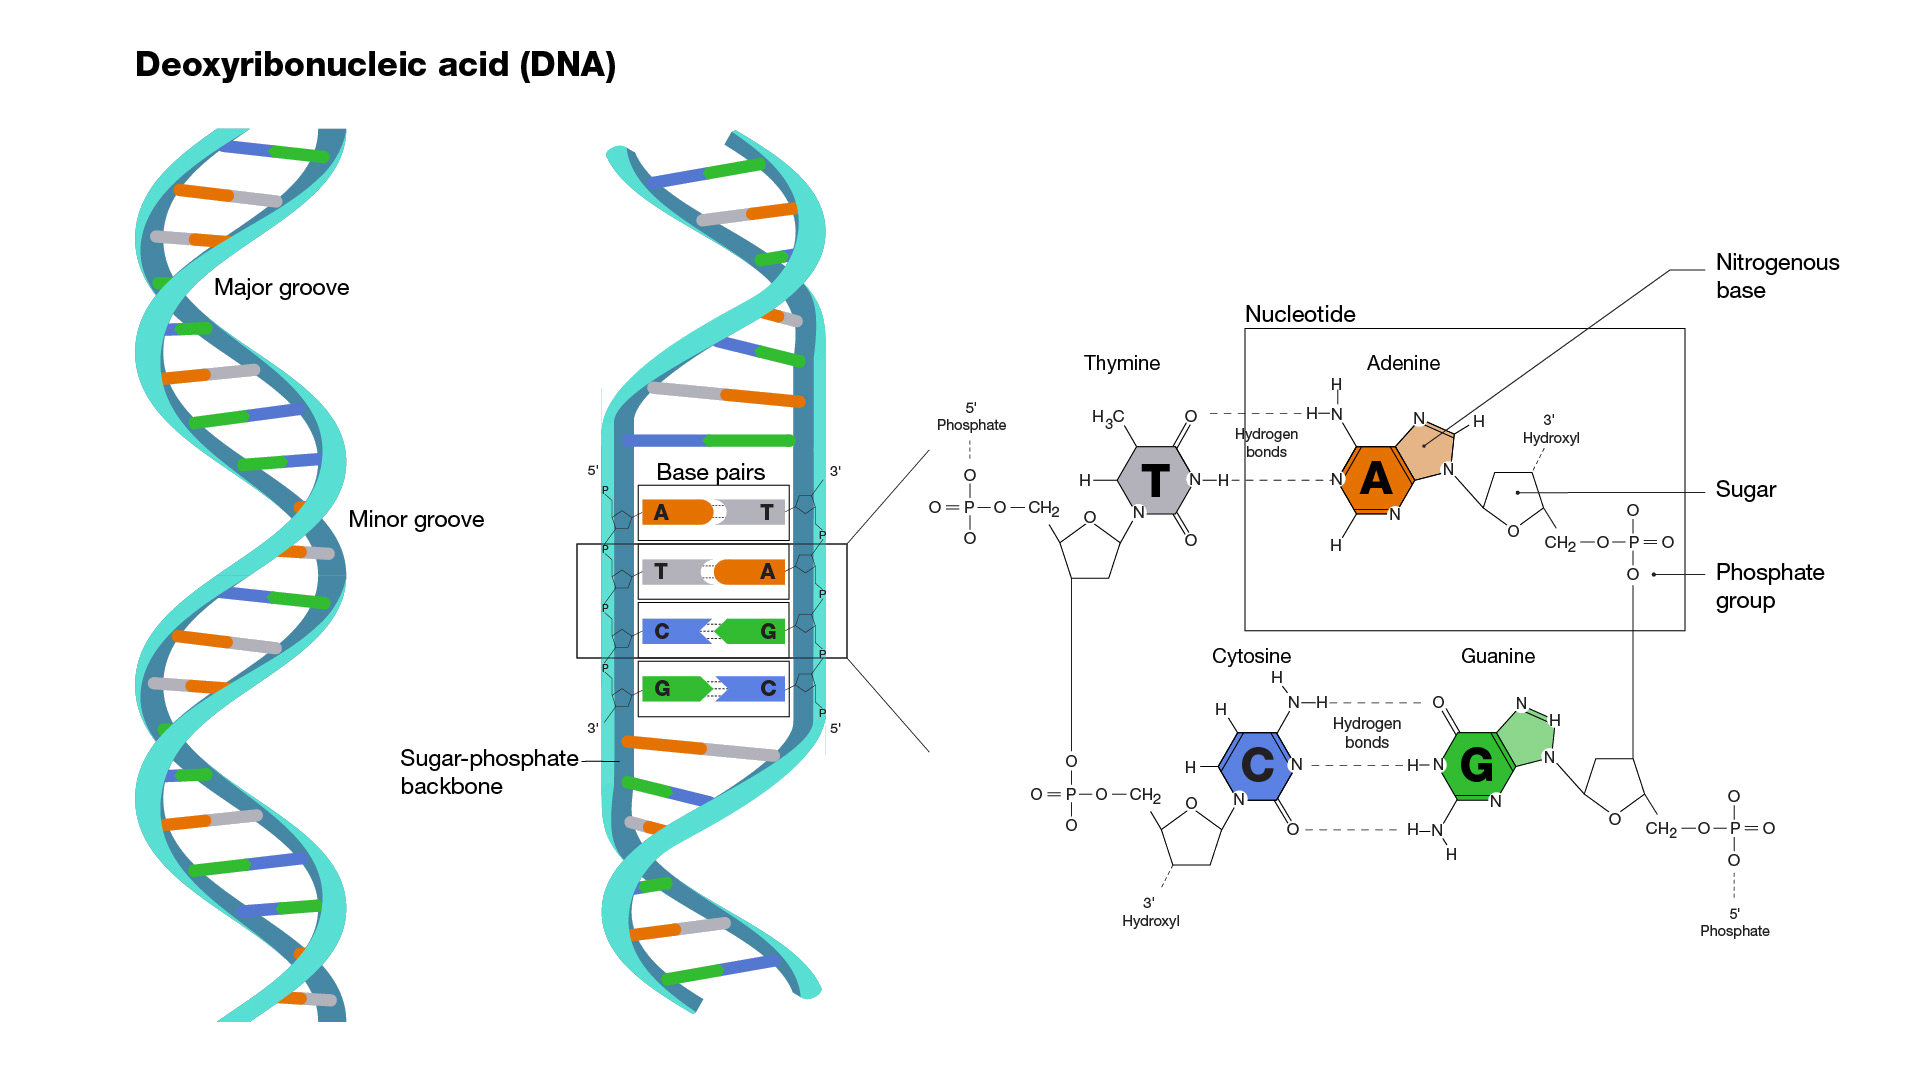
\includegraphics[width=0.6\textwidth]{resources/images/DNA-transparent.png}
  \caption{\textbf{A Diagrammatic Representation of The DNA} double helix structure along with detailed chemical structures of its components \cite{NHGRI2024-DNA}. On the right is the base pairing between nucleotides: specifically, adenine (A) binds with thymine (T), and cytosine (C) binds with guanine (G), all bound by hydrogen bonds.}
  \label{img:dna}
\end{figure}


\begin{wrapfigure}{r}{0.5\textwidth}  
  \centering
  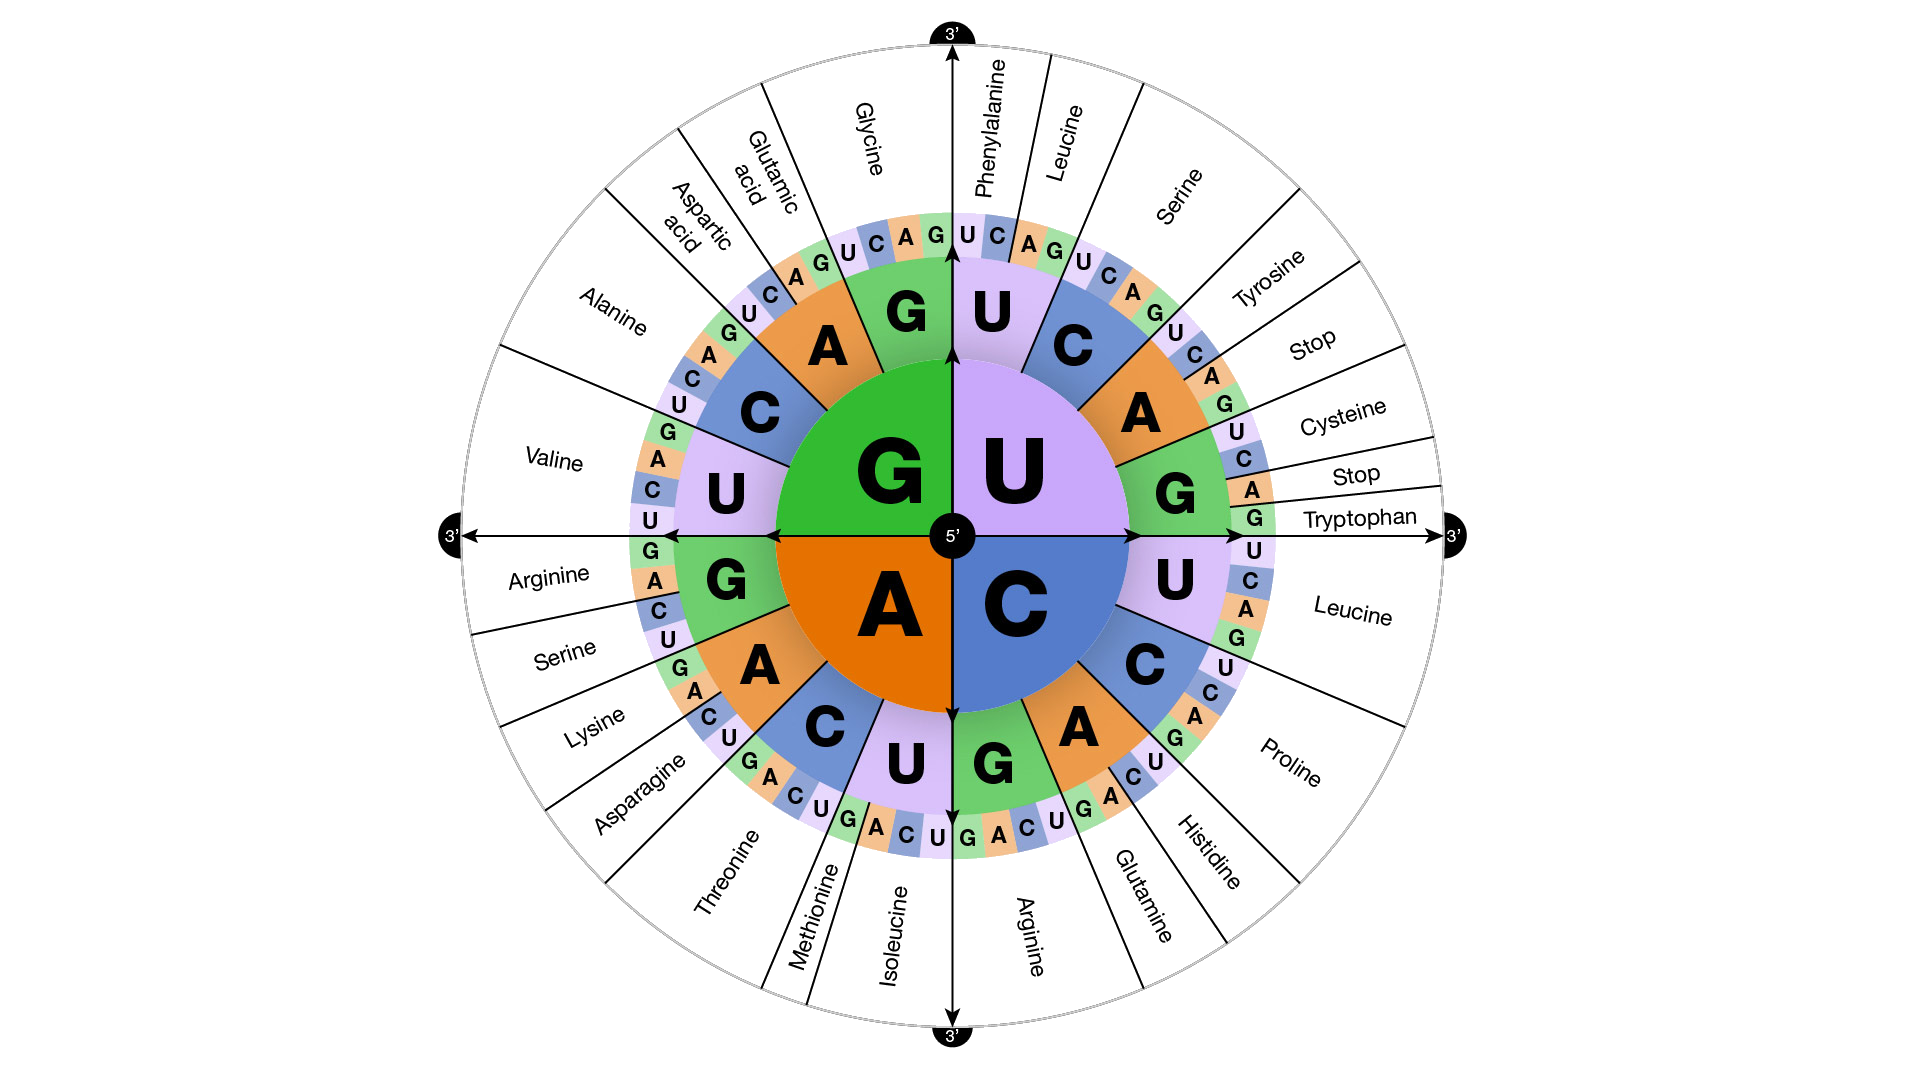
\includegraphics[width=0.48\textwidth]{resources/images/genetic-code.png} 
  \caption{\textbf{Genetic Code}  \cite{NHGRI2024-Code}  details how genes instruct cells to create proteins, using DNA's four bases.}
  \label{img:genetic-code}
\end{wrapfigure}



The \gls{paired-end} (\autoref{img:pe-sequencing}), a technique used in \gls{ngs}, involves sequencing both ends of a \gls{dna} fragment to generate high-quality, alignable sequence data. This method allows for the \gls{sequencing} of both the forward and reverse ends of the fragments, providing two \gls{read}s per fragment. \gls{paired-end} is invaluable for detecting insertions, deletions, and rearrangements, and for improving the \gls{assembly} of complex \gls{genome}s. In the context of this research, \gls{paired-end} can enhance the resolution and accuracy of Mycobacterium tuberculosis genome assemblies by providing more information on the spatial relationships between \gls{dna} fragments, thus facilitating the identification of genomic variations and structural changes.


\begin{figure}[ht]
  \centering
  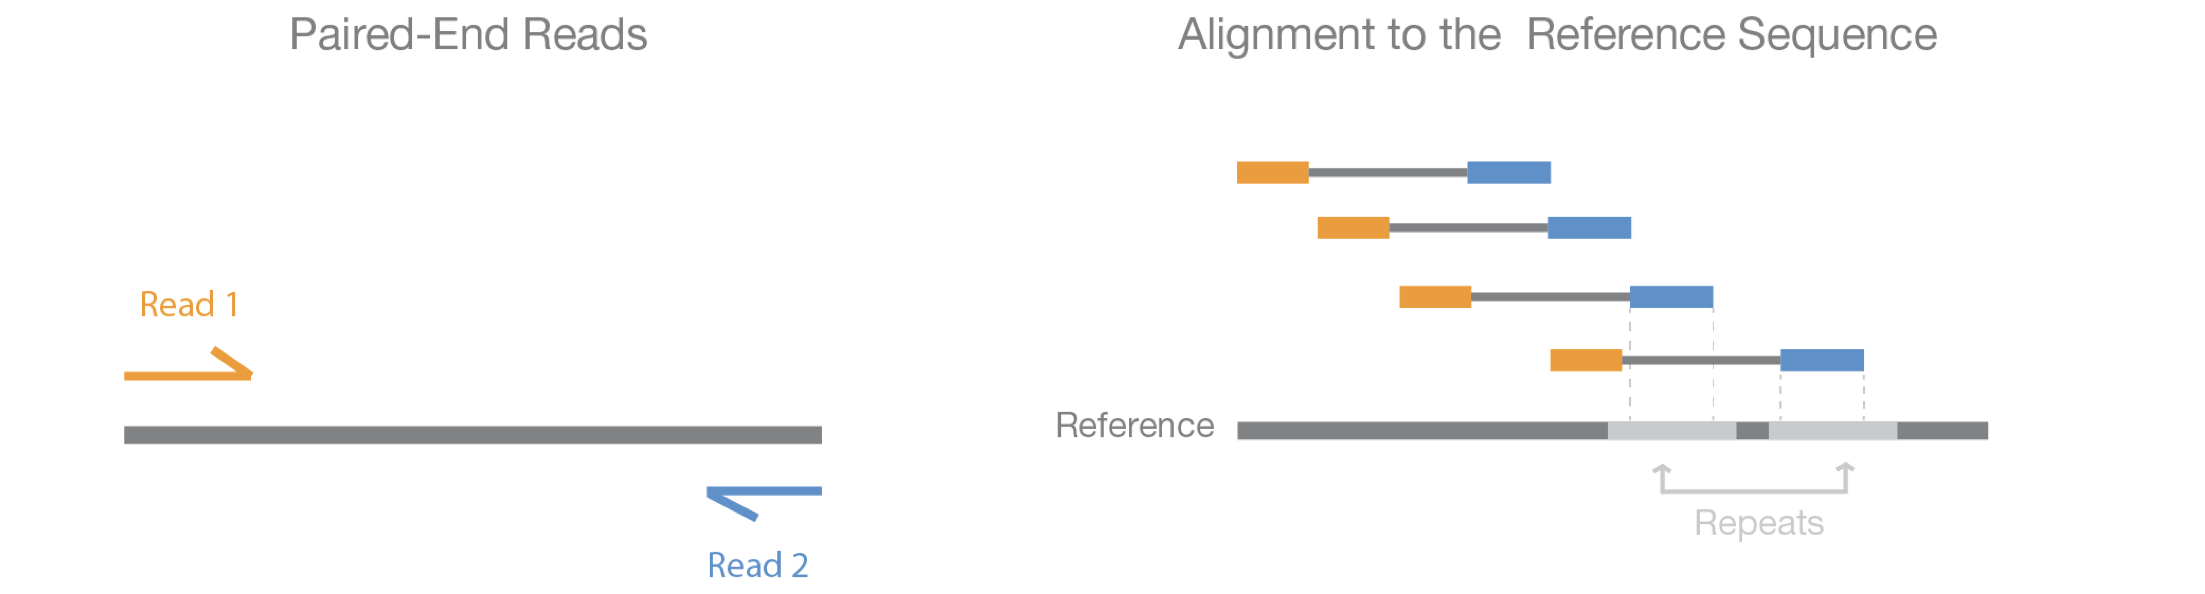
\includegraphics[width=\textwidth]{resources/images/paired-end (PE) sequencing.png}
  \caption{\textbf{Paired-End Sequencing and Alignment} \cite{Illumina2017-PE} — both ends of a DNA fragment are sequenced. The best advantage of this method is that since the distance between each paired read is known, the alignment algorithms can use this information to map the reads over repetitive regions more accurately. This results in better alignment of reads, especially across difficult-to-sequence, repetitive regions of the genome. Sequences aligned as read pairs allow the detection of indels that are not possible with single-read data.}
  \label{img:pe-sequencing}
\end{figure}

\section{Genome Assembly and Quality Assessment}


\begin{SCfigure}[][ht]
  \centering
  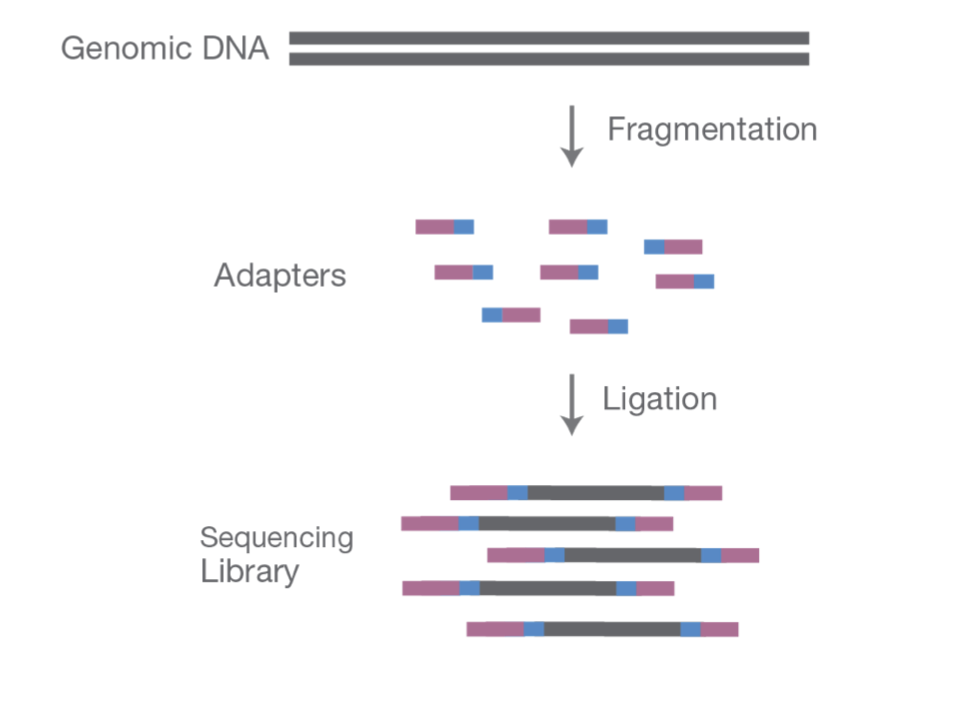
\includegraphics[width=0.48\textwidth]{resources/images/Library Preparation.png}
  \caption{\textbf{Library Preparation} \cite{Illumina2017-LP} — initial sequencing library prep involves breaking DNA into smaller pieces and adding adapters for fragment amplification and sequencing primer attachment.}
  \label{img:library-preparation}
\end{SCfigure}


The \gls{ngs} is a high-throughput methodology that enables rapid \gls{sequencing} of the base pairs in \gls{dna} or RNA samples. \gls{ngs} has largely displaced older methods that were based on electrophoresis, as it is faster, more sensitive, and less expensive to operate. Thus, \gls{ngs} is now used in laboratories ranging from those focused on research on the history of life on Earth to those focused on identifying the exact genetic cause of an individual's disease. The \gls{ngs} workflow follows several key stages, including Library Preparation (\autoref{img:library-preparation}), Cluster Amplification (\autoref{img:cluster-amplification}), \gls{sequencing} (\autoref{img:sequencing}), and Alignment \& Analysis (\autoref{img:alignment-and-analysis}). At each stage, the user's understanding of the nature and details of the genetics of an organism grows, from preparing the selected \gls{dna} or RNA sample in a usable \gls{fastq} \cite{Buffalo2015} to alignment of the \gls{ngs} \gls{read}s and analysis of the data. This process involves aligning and merging fragments from a longer \gls{dna} sequence, resulting in \gls{contig}s and \gls{scaffold}s. The quality of \gls{assembly} is paramount and can be assessed through various \gls{metrics}, such as \gls{n50}, \gls{n90}, \gls{l50}, \gls{l90}, \gls{total length}, \gls{gc}, \gls{largest contigs}, \gls{depth}, and the \gls{n's per 100 kbp}, which give insights into the size and completeness of the assembled \gls{genome}.

\begin{SCfigure}
  \centering
  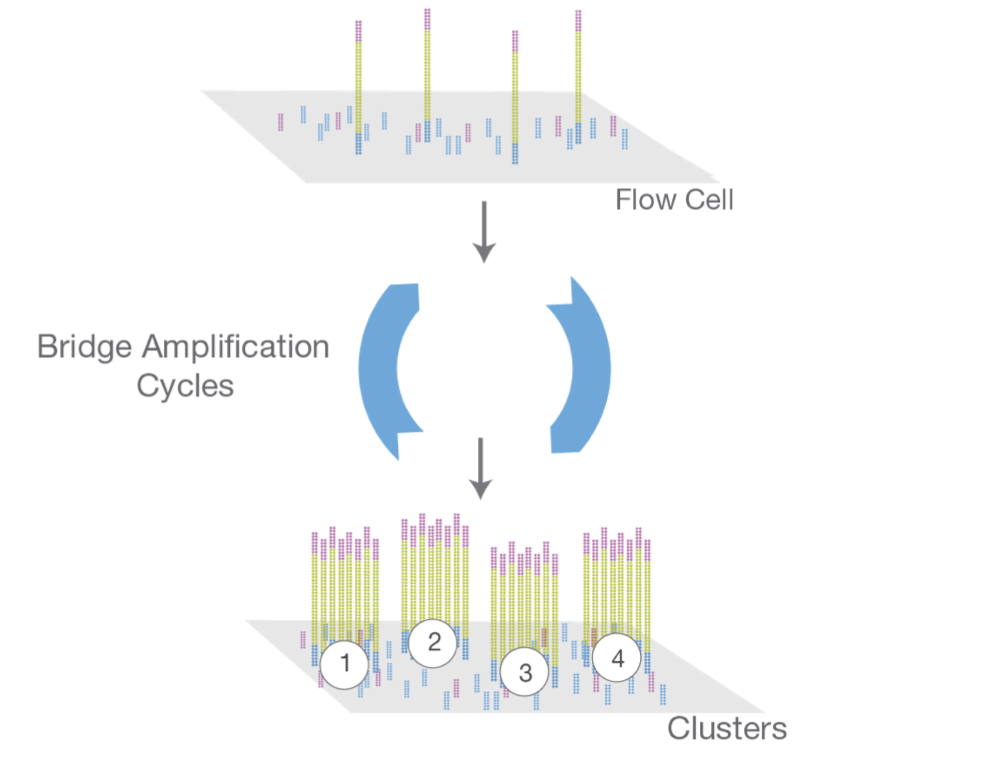
\includegraphics[width=0.48\textwidth]{resources/images/Cluster Amplification.png}
  \caption{\textbf{Cluster Amplification} \cite{Illumina2017-CA} — an image of the bridge amplification process, a crucial step in preparing DNA for sequencing on certain high-throughput platforms, such as Illumina Sequencing Systems. DNA fragments with adapters (blue and pink) ligated to their ends are attached to the flow cell surface (gold).}
  \label{img:cluster-amplification}
\end{SCfigure}

Every stage of high-throughput sequencing relies on robust and efficient methods to derive the \gls{dna} sequence. The first of these steps is the library preparation (\autoref{img:library-preparation}). Genomic \gls{dna} must be processed to be ready for \gls{sequencing}. It is fragmented into small pieces. Adapters are then added to both ends of the fragments. Adapters are short, known \gls{dna} sequences. They have several functions. The first is that they form the priming site for the \gls{sequencing} Process to take place. The adapter also serves as the priming site for the amplification (\autoref{img:cluster-amplification}) of the \gls{dna}. The adapter can also contain a barcode, which allows for the pooling and identification of multiple samples within a single \gls{sequencing} run.

\begin{SCfigure}
  \centering
  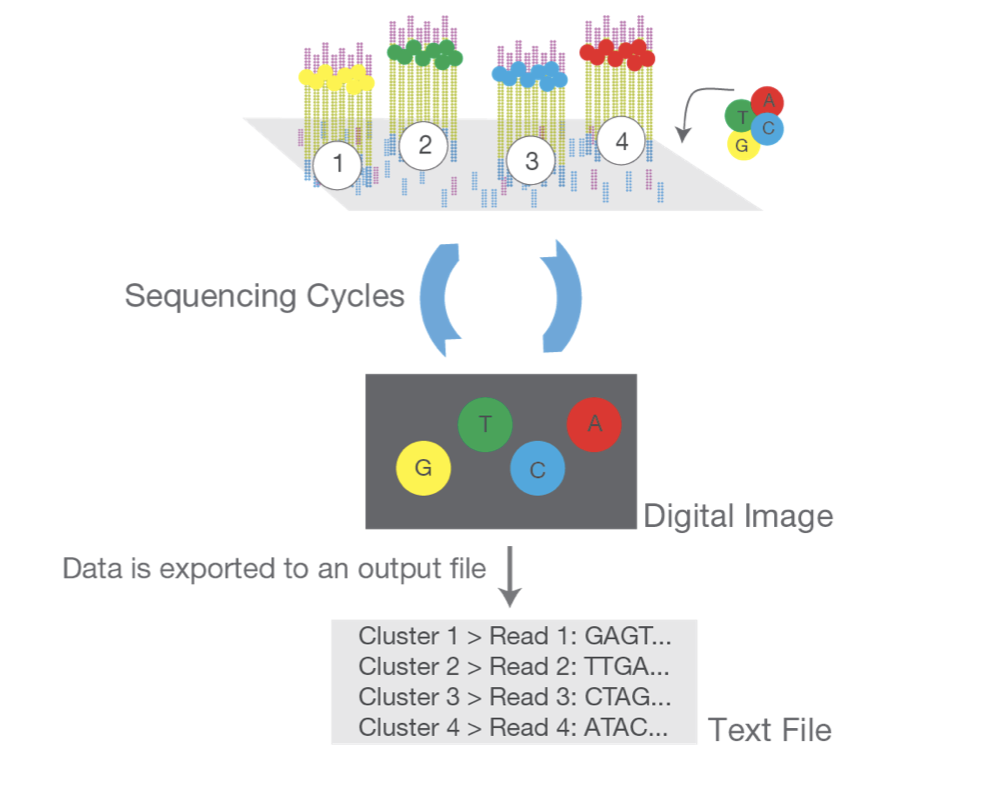
\includegraphics[width=0.48\textwidth]{resources/images/Sequencing.png}
  \caption{\textbf{Sequencing} \cite{Illumina2017-S} — each of the clusters generated from bridge amplification is sequenced one base at a time. A unique fluorescent signal is used to identify each of the four nucleotides (A, T, C, G). As the sequence is built, these signals are captured and translated into a digital image. That digital image is then converted into a text file containing the sequences of the DNA fragments.}
  \label{img:sequencing}
\end{SCfigure}

The library, now ready for attachment to a flow cell (\autoref{img:cluster-amplification}), will undergo clonal amplification on this glass slide. On the surface of the flow cell are lanes that are coated with oligonucleotides that are complementary to the adapters on the fragments. The library is loaded onto the flow cell where the fragments bind to the oligonucleotides. In bridge amplification, the immobilized fragments will bend over and form a bridge and will fragment into oligonucleotides on the other strand. This bridge forms a localized clonal amplification site called a cluster. Within this cluster are many copies of that one DNA.


\begin{SCfigure}
  \centering
  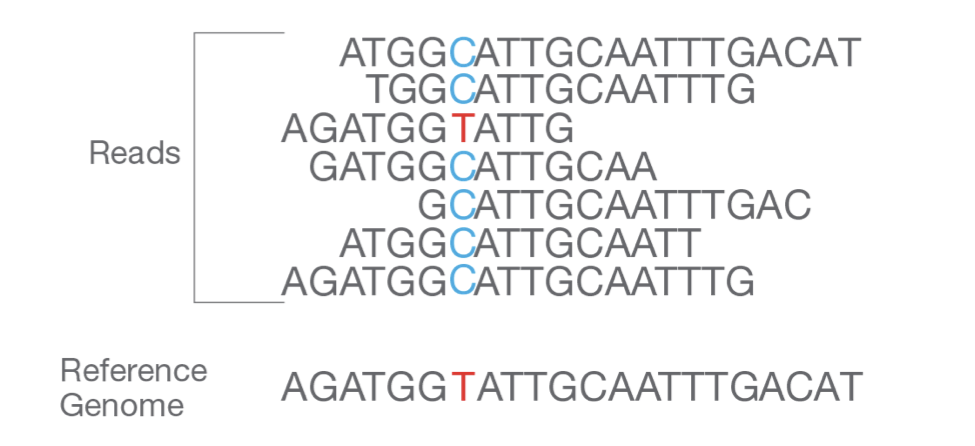
\includegraphics[width=0.48\textwidth]{resources/images/Alignment and Data Analysis.png}
  \caption{\textbf{Alignment \& Analysis} \cite{Illumina2017-ADA} — short DNA sequences (Reads) are matched against a longer ‘Reference Genome’ sequence. The highlighted sections in the Reads indicate a match, or mismatch, to the Reference Sequence.}
  \label{img:alignment-and-analysis}
\end{SCfigure}

The actual \gls{sequencing} (\autoref{img:sequencing}) occurs through a series of cycles. Each cycle adds one nucleotide at a time to the \gls{dna} strand. The nucleotide, or base, is read by a fluorescent signal; the signal is captured and recorded. In this way, chemical information is translated to digital data (each of the four \gls{dna} bases is associated with a unique color). The process cycles, building a sequence read that is complementary to the \gls{dna} template in the library.

Resulting sequence reads are computationally aligned to a Reference \gls{genome} (\autoref{img:alignment-and-analysis}); this process identifies where in the \gls{genome} each \gls{read} comes from and is critical for variant detection and understanding the structure of the \gls{genome}. Additionally, \gls{read}s are assessed for quality; each base call is assigned a quality score, which reflects the confidence of the base call. Ultimately, each analysis reveals variations and mutations, information about genetic predisposition to diseases, and much more.

\section{Impact of Trimming on Assembly Metrics}

The \gls{trimming} in \gls{ngs} is a crucial pre-processing step. During this process, low-quality bases and adapter sequences are carefully removed from \gls{read}s. This significantly affects the quality of the subsequent \gls{assembly}. The effectiveness of different \gls{trimming} Methods \cite{fastp}, such as adapter trimming, quality trimming, and sliding window trimming, can be evaluated based on their impact on important \gls{metrics} like \gls{n50}, \gls{gc} content, and error rates. These techniques are essential to ensure that only high-quality \gls{read}s advance to the \gls{assembly} phase, enhancing the overall accuracy and reliability of genomic analysis.

Moreover, the selection of a \gls{trimming} method can significantly influence downstream analysis and interpretation of \gls{ngs} data. For instance, quality trimming, which focuses on removing bases with low-quality scores, can markedly decrease false positives in variant calling. Conversely, adapter trimming is vital for avoiding artificial chimeras and ensuring the assembly of genuine genomic sequences. The complexities of these methods underscore the importance of a well-thought-out \gls{trimming} strategy, customized to the specific needs of each \gls{ngs} project, to achieve the best results in genomic \gls{sequencing} and analysis.

\section{Data Visualization in Genomic Assembly Analysis}

Data visualization \cite{Chen2007} plays a crucial role in understanding and interpreting the vast amount of data generated by \gls{ngs}.  Visualization tools such as \gls{heatmap}s, \gls{bar}, and \gls{scatter}s can be used to represent various aspects of \gls{assembly} and \gls{trimming} efficiency. For instance, \gls{heatmap}s can illustrate the \gls{deviation} in \gls{read} quality before and after \gls{trimming}, while \gls{bar} can show the relationship between trimming methods and key \gls{metrics} like \gls{n50} and \gls{n's per 100 kbp} \cite{quast}.

\section{Conclusion}

In summary, \gls{ngs} and its associated data analysis techniques, including \gls{trimming} and data visualization, are crucial in assessing \gls{assembly} quality \cite{Wang2022}. Understanding these concepts, as underlined in the recommended literature, provides vital insights into genomic studies, paving the way for advancements in genetics and beyond.
